\cleardoublepage

\chapter{Nodo}
\label{makereference4}

Here are more examples of referring to previous sections.  In
Chapter~\ref{makereference} there were several sections, including
section~\ref{makereference1.1}, section~\ref{makereference1.2},
and section~\ref{makereference1.3}.

Likewise, in Chapter~\ref{makereference2}, there are
sections~\ref{makereference2.1} and ~\ref{makereference2.2}.

\section{Introducción}
\label{makereference4.1}


Como hemos comentado anteriormente el nodo es quien recoge los datos y los envía al servidor de datos.
Para ello, el nodo esta formado por una Raspberry Pi modelo 2b con Raspbian a la que están conectados dos sensores: DHT22 (temperatura y humedad) y un piranómetro~\ref{figure2}.

Gracias a la ayuda de los 'datasheets' proporcionados por los fabricantes de los dispositivos, comprendimos cómo era el funcionamiento de estos. 
Las llamadas al sensor se realizan a través de su API en Python, proporcionada por Adafruit, lo cual nos facilitó mucho el trabajo de recolección de datos.

En el nodo corre un script que se encarga de recoger los datos del exterior y enviarlos vía MQTT al servidor de datos para, más adelante, ser procesados.

-----
http://www.pveducation.org/pvcdrom/2-properties-sunlight/solar-radiation-earths-surface

La radiación solar varía debido a diversos factores, como los efectos atmosféricos, las variaciones locales en la atmósfera como el vapor de agua, las nubes y la contaminación, otros como la latitud y la estación del año y la hora del día.

---https://www.imn.ac.cr/documents/10179/27818/factores-influyen-radiac-UV.pdf/187e5ea7-7c11-4ed7-955b-4e35c2f0ebf1

Por ejemplo la latitud influye en la cantidad de radiación solar que llega a la superficie; por otro lado la radiación disminuirá cuanta más cantidad de nubes y más alta sea la humedad. Al contrario pasará con la temperatura, cuanto más altas sean las temperaturas mayor sera la radiación. Otro factor que influye a la hora de medir la radiación es el tipo de superficie, porque la reflexión de los rayos varía según el tipo de superficie, la nieve se refleja un 85 por ciento, al contrario del asfalto que solo un 2 por ciento.

Hay otros elementos que podríamos haber medido y que no lo hemos hecho,como los comentados anteriormente o por ejemplo también la velocidad del viento, que nos importaría si refrigera el panel.
Como hemos dicho a superficie y la altitud es otro de estos elementos, aunque este está a su vez relacionado con la temperatura, ya que por ejemplo cuando nosotros lo hemos sacado para hacer las pruebas, rápidamente es alcanzado por el sol y alcanza altas temperaturas, no es igual que si está en la superficie.

Por lo que decidimos limitarnos a recoger información de radiación y temperatura porque son las más relevantes para nuestro modelo.


\begin{figure}[htb]
	
	\begin{center}
		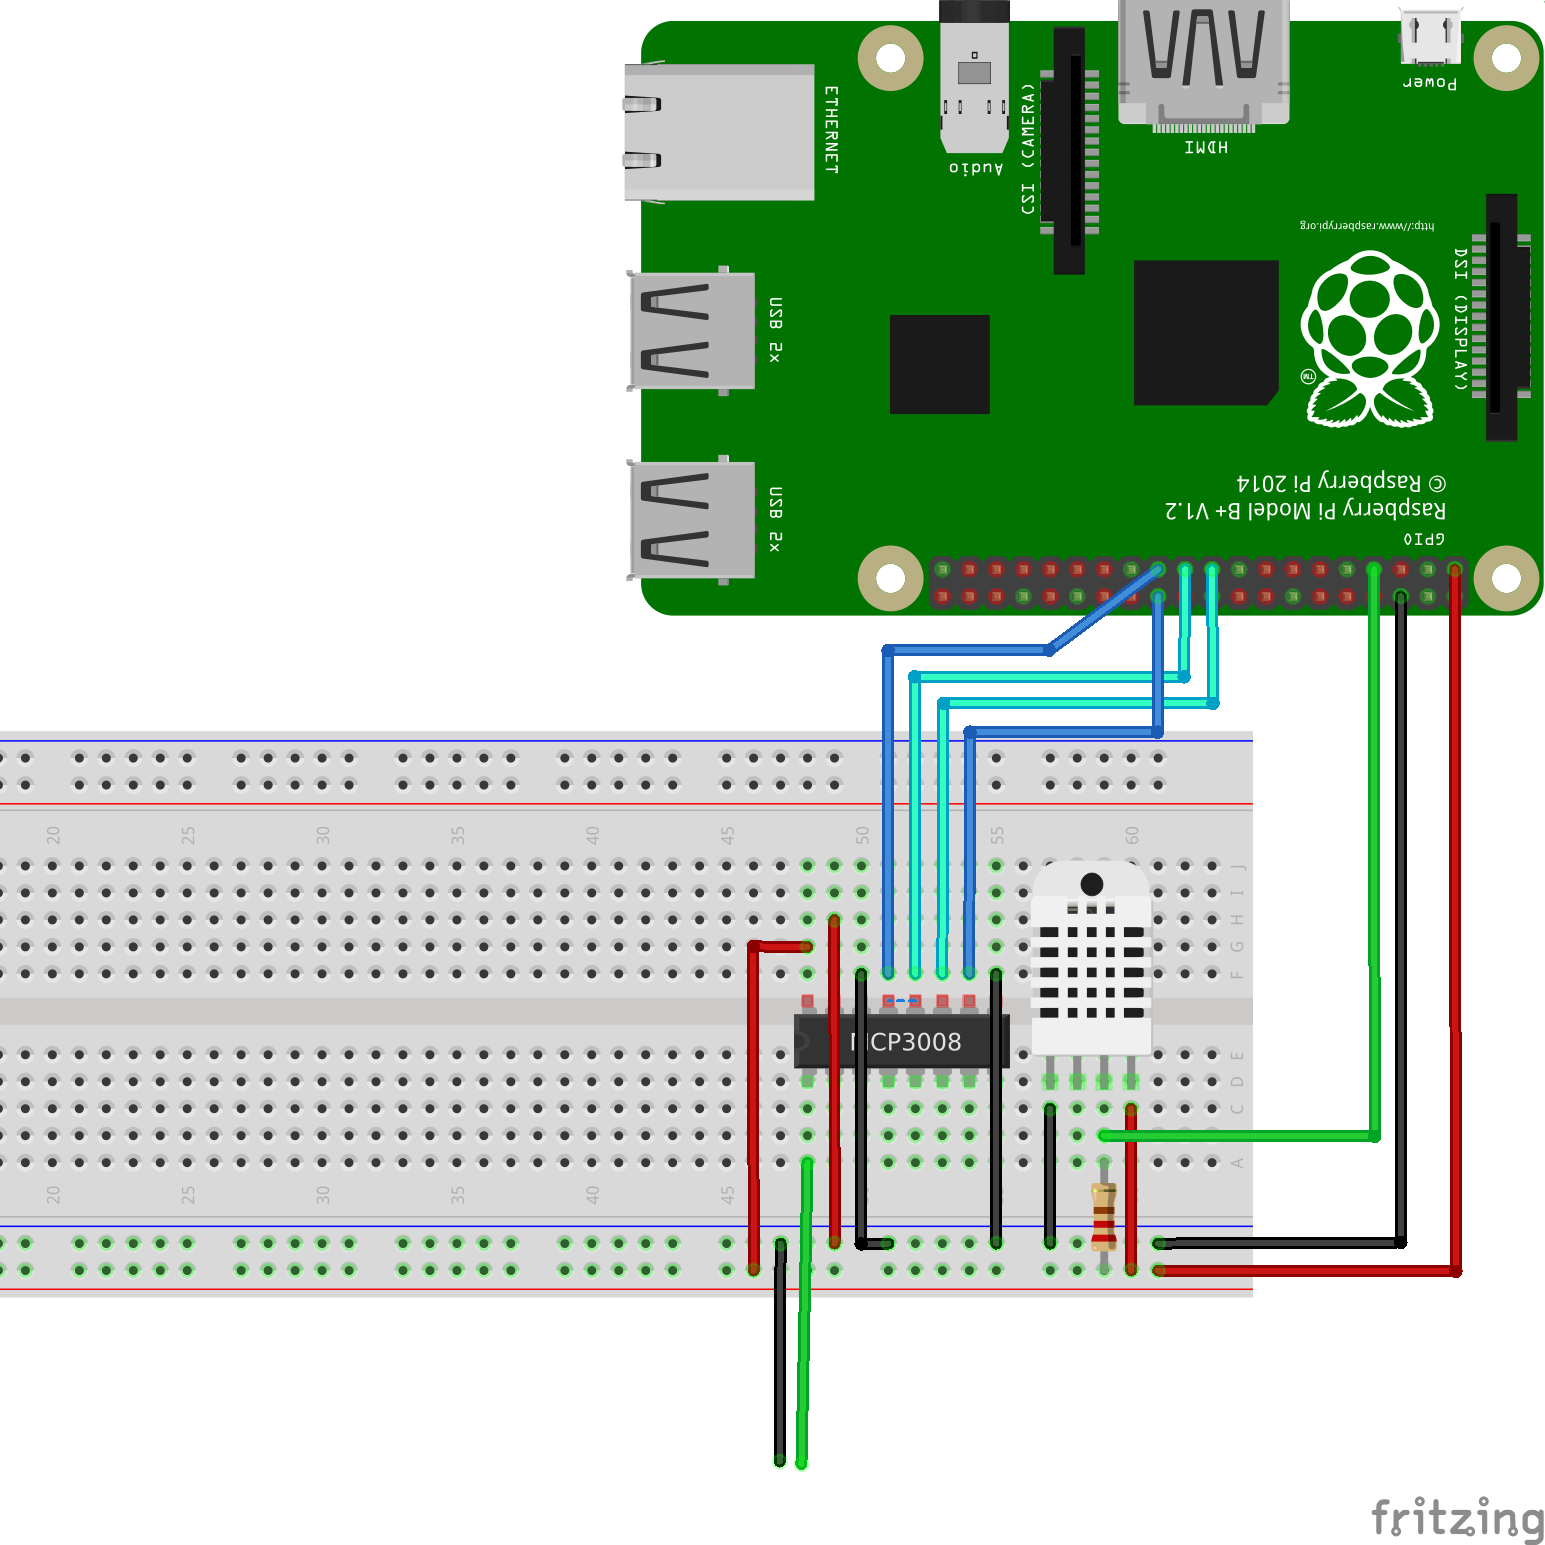
\includegraphics[width=15cm,height=15cm]{figures/solar_project_node_diagram.png}
		\caption{Diagrama del nodo}
	\end{center}
	
	\label{figure2}
\end{figure}

\section{Elementos utilizados}
\label{makereference4.2}
\subsection{Raspberry}

Nuestro nodo esta formado por una Raspberry Pi que es un "pequeño ordenador", un computador de placa reducida   \ref{figure3}. Se dice que es un pequeño ordenador porque soporta componentes de un ordenador pero es una pequeña placa, con el cual podemos hasta jugar como en un ordenador normal o conectar un teclado y una pantalla.
 Raspbian es una versión adaptada de Debian y es su sistema operativo oficial, pero permite otros.
 
 \begin{figure}[htb]
 	
 	\begin{center}
 		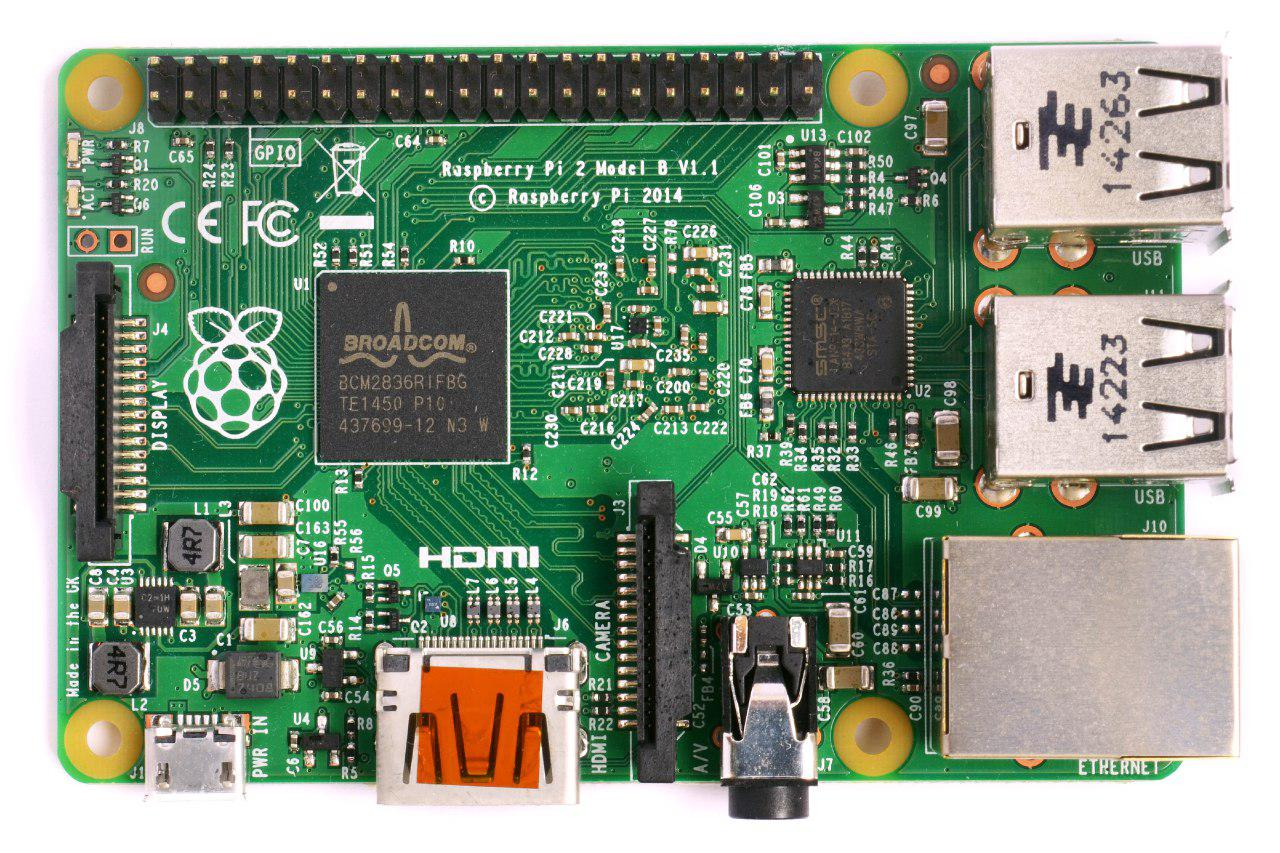
\includegraphics[width=12cm,height=10cm]{figures/Raspberry_Pi.jpg}
 		\caption{Raspberry Pi Modelo 2b}
 	\end{center}
 	
 	\label{figure3}
 \end{figure}
 
Fue creado en 2006, en la Universidad de Cambridge, con el fin de fomentar la enseñanza en las escuela de ciencias de la computación, pero hasta 2012 no salió al mercado.

Existen distintos modelos de Raspberry Pi, desde la Raspberry Pi 1 Modelo A hasta la Raspberry Pi 3 Modelo B \ref{figure4}.
En nuestro proyecto hemos usado una Raspberry Pi modelo 2b, con su sistema operativo oficial , Raspbian.


 \begin{figure}[htb]
	
	\begin{center}
		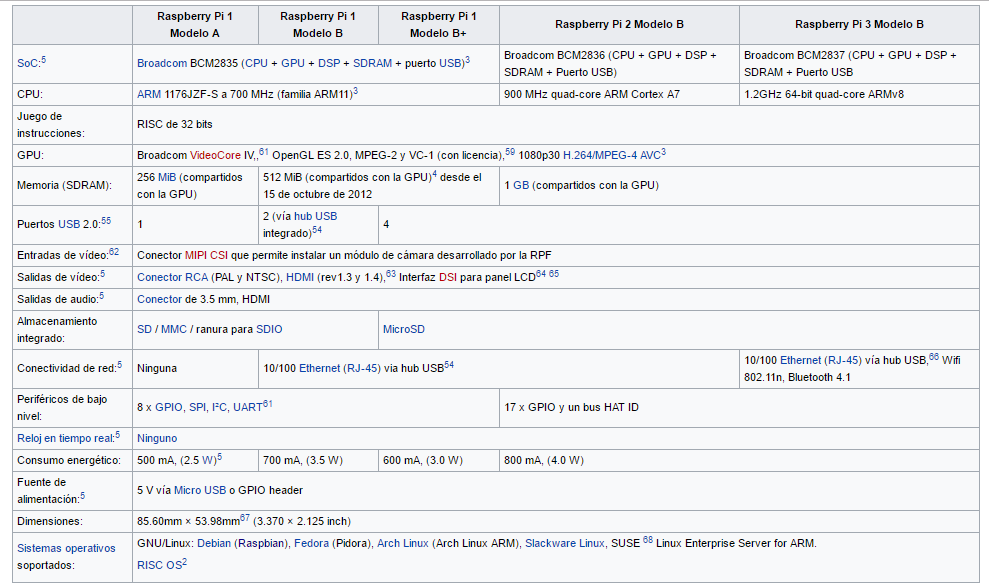
\includegraphics[width=17cm,height=17cm]{figures/Cuadro_Tipos_Raspberry.png}
		\caption{Cuadro comparativo de las especificaciones técnicas}
	\end{center}
	
	\label{figure4}
\end{figure}


Sabemos que hay otros nodos muchos más baratos, con menos consumo, menos capacidad y más fácil para prototipado, pero como no es la placa final, decidimos que para un primer prototipo está muy bien, porque es relativamente barata para hacer un nodo, para hacer muchos no, pero para uno solo sí. Además como tiene sistema operativo, facilita el desarrollo, puedes depurar. Y como es ampliamente usada y existe una comunidad, ayuda que a la hora de tener un problema siempre tiendes donde consultar.



\subsection{Sensor de temperatura y humedad}

Nuestro nodo tiene conectado en la Raspberry dos sensores, uno de temperatura y humedad y un piranómetro del cual hablaremos más tarde, ambos para recoger los datos meteorológicos que necesitamos para nuestro modelo.

Normalmente en los modelos que predicen lo que va a producir un panel solar, los elementos que más afecta son, por supuesto la radiación, pero también la temperatura, ya que a mayor temperatura el panel es menos eficaz. 

--https://www.luisllamas.es/arduino-dht11-dht22/

El sensor que hemos utilizado para medir la temperatura y humedad es un sensor DHT22, y permite medir simultáneamente ambos parámetros. 
Este sensor tiene un procesador interno que es el que realiza la medición y la proporciona mediante una señal digital.
Algunas de las características de este sensor y en especial de este modelo, ya que tambien existe el modelo DHT11, son que tiene una precisión de 0.5ºC para medir la temperatura, y entre un 2 y un 5 por ciento para la humedad. Ademas recoge 2 muestras por segundo. Este sensor no es un sensor de alta precisión, pero es suficiente para nuestro proyecto, además de tener un precio muy económico \ref{figure4}.

 \begin{figure}[htb]
	
	\begin{center}
		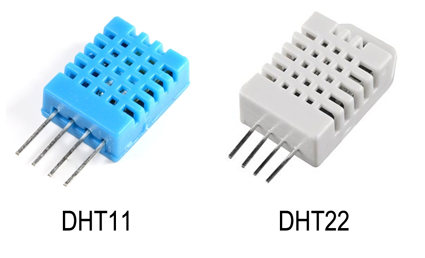
\includegraphics[width=7cm,height=7cm]{figures/sensorTemperaturaHumedad.png}
		\caption{Sensores de temperatura y humedad DHT11 y DHT22}
	\end{center}
	
	\label{figure5}
\end{figure} 

\subsection{Piranómetro}


\section{Organización del código}
\label{makereference4.3} 
	\subsection{Librerías usadas}
		\subsubsection{Adafruit}
		Adafruit es una compañía de hardware open-source, que además de proporcionar hardware, suministra de una gran cantidad de documentación y librerías para facilitar el trabajo con sus componentes.
		
		\subsubsection{Pandas}
		Pandas es una biblioteca de software escrita para Python para la manipulación y análisis de datos. En particular, ofrece estructuras de datos y operaciones para manipular tablas numéricas y series temporales.
		
		\subsubsection{Paho}
		El proyecto Paho ha sido creado para proporcionar implementaciones escalables de código abierto de protocolos de mensajería abiertos y estándar dirigidos a aplicaciones nuevas, existentes y emergentes para Machine to Machine (M2M) e Internet of Things (IoT).
		
		Paho refleja las restricciones inherentes físicas y de costo de la conectividad del dispositivo. Los objetivos incluyen niveles efectivos de desacoplamiento entre dispositivos y aplicaciones, diseñados para mantener los mercados abiertos y fomentar el rápido crecimiento de middleware y aplicaciones escalables de Web y Enterprise. Paho inicialmente comenzó con implementaciones de cliente de publicación / suscripción de MQTT para su uso en plataformas incrustadas, y en el futuro traerá el soporte de servidor correspondiente según lo determinado por la comunidad.
		
	\subsection{Flujo de datos}

\section{Método de instalación y puesta en marcha}
\label{makereference4.4}